\chapter{Potential Formulation and Radiation-Solutions}
\begin{abox}
	Practise Set-1
\end{abox}
\begin{enumerate}
	\item   For constant uniform electric and magnetic field $\vec{E}=\vec{E}_{0}$ and $\vec{B}=\vec{B}_{0}$, it is possible to choose a gauge such that the scalar potential $\phi$ and vector potential $\vec{A}$ are given by
	{\exyear{NET/JRF(JUNE-2011)}}
	\begin{tasks}(2)
		\task[\textbf{a.}] $\phi=0$ and $\vec{A}=\frac{1}{2}\left(\vec{B}_{0} \times \vec{r}\right)$
		\task[\textbf{b.}] $\phi=-\vec{E}_{0} \cdot \vec{r}$ and $\vec{A}=\frac{1}{2}\left(\vec{B}_{0} \times \vec{r}\right)$
		\task[\textbf{c.}]  $\phi=-\vec{E}_{0} \cdot \vec{r}$ and $\vec{A}=0$
		\task[\textbf{d.}] $\phi=0$ and $\vec{A}=-\vec{E}_{0} t$
	\end{tasks}
	\begin{answer}
		\begin{align*}
		\text{Let }\vec{E}&=E_{0}(\hat{x}+\hat{y}+\hat{z})\text{ and } \vec{B}\\&=B_{0}(\hat{x}+\hat{y}+\hat{z})\text{ since they are constant vector.}\\
		\text{Lorentz Gauge condition is }\vec{\nabla} \cdot \vec{A}&=-\mu_{0} \varepsilon_{0} \frac{\partial \phi}{\partial t}\\
		\intertext{	$\left\{\right.$ since $\left.\vec{B} \times \vec{r}=B_{0}(z-y) \hat{x}-B_{0}(z-x) \hat{y}+B_{0}(y-x) \hat{z}\right\}$}
		\end{align*}
		So the correct answer is \textbf{Option (a)}
	\end{answer}
	\item	 A constant electric current $I$ in an infinitely long straight wire is suddenly switched on at $t=0$. The vector potential at a perpendicular distance $r$ from the wire is given by $\vec{A}=\frac{\hat{k} \mu_{0} I}{2 \pi} \ln \left[\frac{1}{r}\left(c t+\sqrt{c^{2} t^{2}-r^{2}}\right)\right]$. The electric field at a distance $r(<c t)$ is
	{\exyear{NET/JRF(DEC-2011)}}
	\begin{tasks}(2)
		\task[\textbf{a.}] 0
		\task[\textbf{b.}] $\frac{\mu_{0} I}{2 \pi t} \frac{1}{\sqrt{2}}(\hat{i}-\hat{j})$
		\task[\textbf{c.}] $\frac{c \mu_{0} I}{2 \pi \sqrt{c^{2} t^{2}-r^{2}}} \frac{1}{\sqrt{2}}(\hat{i}+\hat{j})$
		\task[\textbf{d.}] $-\frac{c \mu_{0} I}{2 \pi \sqrt{c^{2} t^{2}-r^{2}}} \hat{k}$
	\end{tasks}
\begin{answer}
	\begin{align*}
	\vec{E}&=-\vec{\nabla} \phi-\frac{\partial \vec{A}}{\partial t}=-\frac{\partial \vec{A}}{\partial t} \Rightarrow \vec{E}\\&=-\frac{\mu_{0} I}{2 \pi}\frac{r}{\left(c t+\sqrt{c^{2} t^{2}-r^{2}}\right)}\left[\frac{1}{r}\left(c+\frac{2 c^{2} t}{2 \sqrt{c^{2} t^{2}-r^{2}}}\right)\right]\\
	\Rightarrow \vec{E}&=\frac{-c \mu_{0} I}{2 \pi \sqrt{c^{2} t^{2}-r^{2}}} \hat{k}
	\end{align*}
	So the correct answer is \textbf{Option (d)}
\end{answer}
	\item  Consider an infinite conducting sheet in the $x y$-plane with a time dependent current density $K t \hat{i}$, where $K$ is a constant. The vector potential at $(x, y, z)$ is given by $\vec{A}=\frac{\mu_{0} K}{4 c}(c t-z)^{2} \hat{i}$. The magnetic field $\vec{B}$ is
	{	\exyear{NET/JRF(DEC-2012)}}
	\begin{tasks}(2)
		\task[\textbf{a.}] $\frac{\mu_{0} K t}{2} \hat{j}$
		\task[\textbf{b.}] $-\frac{\mu_{0} K z}{2 c} \hat{j}$
		\task[\textbf{c.}] $-\frac{\mu_{0} K}{2 c}(c t-z) \hat{i}$
		\task[\textbf{d.}] $-\frac{\mu_{0} K}{2 c}(c t-z) \hat{j}$
	\end{tasks}
\begin{answer}
	\begin{align*}
	\vec{B}&=\vec{\nabla} \times \vec{A}=\frac{\partial A_{x}}{\partial z} \hat{y}=-\frac{\mu_{0} K}{2 c}(c t-z) \hat{j}
	\end{align*}
	So the correct answer is \textbf{Option (d)}
\end{answer}
	\item  A current $I$ is created by a narrow beam of protons moving in vacuum with constant velocity $\vec{u}$. The direction and magnitude, respectively of the Poynting vector $\vec{S}$ outside the beam at a radial distance $r$ (much larger than the width of the beam) from the axis, are
	{	\exyear{NET/JRF(JUNE-2013)}}
	\begin{tasks}(2)
		\task[\textbf{a.}] $\vec{S} \perp \vec{u}$ and $|\vec{S}|=\frac{I^{2}}{4 \pi^{2} \varepsilon_{0}|\vec{u}| r^{2}}$
		\task[\textbf{b.}] $\vec{S} \|(-\vec{u})$ and $|\vec{S}|=\frac{I^{2}}{4 \pi^{2} \varepsilon_{0}|\vec{u}| r^{4}}$
		\task[\textbf{c.}] $\vec{S} \| \vec{u}$ and $|\vec{S}|=\frac{I^{2}}{4 \pi^{2} \varepsilon_{0}|\vec{u}| r^{2}}$
		\task[\textbf{d.}] $\vec{S} \| \vec{u}$ and $|\vec{S}|=\frac{I^{2}}{4 \pi^{2} \varepsilon_{0}|\vec{u}| r^{4}}$
	\end{tasks}
\begin{answer}
	\begin{align*}
	\intertext{Let charge per unit length be $\lambda$, hence $I=\lambda u$ in $z$-direction.}
	\text{The magnetic field at a distance $r$ is }\vec{B}&=\frac{\mu_{0} I}{2 \pi r} \hat{\phi}.\\
	\text{The electric field at a distance $r$ is }\vec{E}&=\frac{\lambda}{2 \pi \varepsilon_{0} r} \hat{r}=\frac{I}{2 \pi \varepsilon_{0} u r} \hat{r}.\\
	\text{Hence Poynting vector }\vec{S}&=\frac{\vec{E} \times \vec{B}}{\mu_{0}}=\frac{I^{2}}{4 \pi^{2} \varepsilon_{0} u r^{2}} \hat{z}
	\end{align*}
	So the correct answer is \textbf{Option (c)}
\end{answer}
	\item
	 If the electric and magnetic fields are unchanged when the potential $\vec{A}$ changes (in suitable units) according to $\vec{A} \rightarrow \vec{A}+\hat{r}$, where $\vec{r}=r(t) \hat{r}$, then the scalar potential $\Phi$ must simultaneously change to
	{	\exyear{NET/JRF(JUNE-2013)}}
	\begin{tasks}(4)
		\task[\textbf{a.}] $\Phi-r$
		\task[\textbf{b.}] $\Phi+r$
		\task[\textbf{c.}] $\Phi-\partial \mathrm{r} / \partial t$
		\task[\textbf{d.}] $\Phi+\partial \mathrm{r} / \partial t$
	\end{tasks}
\begin{answer}
	\begin{align*}
	\overrightarrow{A^{\prime}}&=\vec{A}+\vec{\nabla} \lambda=\vec{A}+\hat{r} \Rightarrow \partial \lambda / \partial r=1 \Rightarrow \lambda=r+C\\
	V^{\prime}&=V-\partial \lambda / \partial t=V-\partial r / \partial t
	\end{align*}
	So the correct answer is \textbf{Option (c)}
\end{answer}
	\item
	 Let $(V, \vec{A})$ and $\left(V^{\prime}, \overrightarrow{A^{\prime}}\right)$ denote two sets of scalar and vector potentials, and $\psi$ is a scalar function. Which of the following transformations leave the electric and magnetic fields (and hence Maxwell's equations) unchanged?
	{\exyear{NET/JRF(DEC-2013)}}
	\begin{tasks}(2)
		\task[\textbf{a.}] $\overrightarrow{A^{\prime}}=\vec{A}+\nabla \psi$ and $V^{\prime}=V-\frac{\partial \psi}{\partial t}$
		\task[\textbf{b.}] $\overrightarrow{A^{\prime}}=\vec{A}-\nabla \psi$ and $V^{\prime}=V+2 \frac{\partial \psi}{\partial t}$
		\task[\textbf{c.}] $\overrightarrow{A^{\prime}}=\vec{A}+\nabla \psi$ and $V^{\prime}=V+\frac{\partial \psi}{\partial t}$
		\task[\textbf{d.}] $\overrightarrow{A^{\prime}}=\vec{A}-\nabla \psi$ and $V^{\prime}=V-\frac{\partial \psi}{\partial t}$
	\end{tasks}
\begin{answer}
	So the correct answer is \textbf{Option (a)}
\end{answer}
	\item
	 A time-dependent current $\vec{I}(t)=K t \hat{z}$ (where $K$ is a constant) is switched on at $t=0$ in an infinite current-carrying wire. The magnetic vector potential at a perpendicular distance $a$ from the wire is given (for time $t>a / c$ ) by
	{	\exyear{NET/JRF(JUNE-2014)}}
	\begin{tasks}(2)
		\task[\textbf{a.}]  $\hat{z} \frac{\mu_{0} K}{4 \pi c} \int_{-\sqrt{c^{2} t^{2}-a^{2}}}^{\sqrt{c^{2} t^{2}-a^{2}}} d z \frac{c t-\sqrt{a^{2}+z^{2}}}{\left(a^{2}+z^{2}\right)^{1 / 2}}$
		\task[\textbf{b.}]  $\hat{z} \frac{\mu_{0} K}{4 \pi} \int_{-c t}^{c t} d z \frac{t}{\left(a^{2}+z^{2}\right)^{1 / 2}}$
		\task[\textbf{c.}] $\hat{z} \frac{\mu_{0} K}{4 \pi c} \int_{-c t}^{c t} d z \frac{c t-\sqrt{a^{2}+z^{2}}}{\left(a^{2}+z^{2}\right)^{1 / 2}}$
		\task[\textbf{d.}] $\hat{z} \frac{\mu_{0} K}{4 \pi} \int_{-\sqrt{c^{2} t^{2}-a^{2}}}^{\sqrt{c^{2} t^{2}-a^{2}}} d z \frac{t}{\left(a^{2}+z^{2}\right)^{1 / 2}}$
	\end{tasks}
	\begin{answer}$\left. \right. $
		\begin{figure}[H]
			\centering
			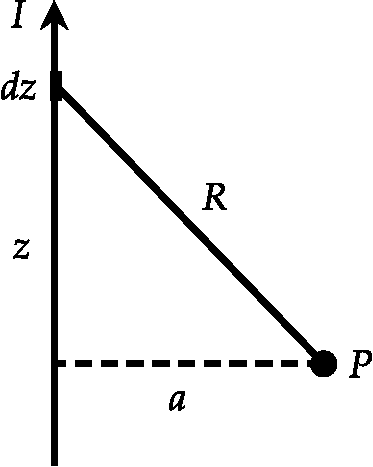
\includegraphics[height=4.5cm,width=3.5cm]{diagram-20211011(26)-crop}
		\end{figure}
		\begin{align*}
		\vec{A}&=\hat{z} \frac{\mu_{0}}{4 \pi} \int_{-\infty}^{\infty} \frac{I\left(t_{r}\right)}{R} d z=\hat{z} \frac{\mu_{0}}{4 \pi} \int_{-\infty}^{\infty} \frac{K(t-R / c)}{R} d z\\
		\Rightarrow \vec{A}&=\hat{z} \frac{\mu_{0} K}{4 \pi c} \int_{-\sqrt{c^{2} t^{2}-a^{2}}}^{\sqrt{c^{2} t^{2}-a^{2}}} d z \frac{c t-\sqrt{a^{2}+z^{2}}}{\left(a^{2}+z^{2}\right)^{1 / 2}}
		\end{align*}
		So the correct answer is \textbf{Option (a)}
	\end{answer}
	\item  The vector potential $\vec{A}=k e^{-a t} r \hat{r}$ (where $a$ and $k$ are constants) corresponding to an electromagnetic field is changed to $\overrightarrow{A^{\prime}}=-k e^{-a t} r \hat{r}$. This will be a gauge transformation if the corresponding change $\phi^{\prime}-\phi$ in the scalar potential is
	{\exyear{NET/JRF(JUNE-2017)}}
	\begin{tasks}(4)
		\task[\textbf{a.}] $a k r^{2} e^{-a t}$
		\task[\textbf{b.}] $2 a k r^{2} e^{-a t}$
		\task[\textbf{c.}] $-a k r^{2} e^{-a t}$
		\task[\textbf{d.}] $-2 a k r^{2} e^{-a t}$
	\end{tasks}
\begin{answer}
	\begin{align*}
	\intertext{Gauge TransformationGauge Transformation}
	\vec{A}&=\vec{A}+\vec{\nabla} \lambda, \phi^{\prime}=\phi-\frac{\partial \lambda}{\partial t} \Rightarrow \vec{A}-\vec{A}\\&=-2 k e^{-a t} r \hat{r}=\vec{\nabla} \lambda=\frac{\partial \lambda}{\partial r} \hat{r}\\
	\Rightarrow \lambda&=-k e^{-a t} r^{2} \Rightarrow \frac{\partial \lambda}{\partial t}=k a e^{-a t} r^{2}\\
	\Rightarrow \phi^{\prime}-\phi&=-\frac{\partial \lambda}{\partial t}=-k a e^{-a t} r^{2}
	\end{align*}
	So the correct answer is \textbf{Option (c)}
\end{answer}
	\item  The charge distribution inside a material of conductivity $\sigma$ and permittivity $\in$ at initial time $t=0$ is $\rho(r, 0)=\rho_{0}$, a constant. At subsequent times $\rho(r, t)$ is given by
	{\exyear{NET/JRF(JUNE-2017)}}
	\begin{tasks}(2)
		\task[\textbf{a.}]  $\rho_{0} \exp \left(-\frac{\sigma t}{\epsilon}\right)$
		\task[\textbf{b.}] $\frac{1}{2} \rho_{0}\left[1+\exp \left(\frac{\sigma t}{\in}\right)\right]$
		\task[\textbf{c.}]  $\frac{\rho_{0}}{\left[1-\exp \left(\frac{\sigma t}{\epsilon}\right)\right]}$
		\task[\textbf{d.}] $\rho_{0} \cosh \frac{\sigma t}{\in}$
	\end{tasks}
\begin{answer}
	\begin{align*}
	\vec{J}_{f}&=\sigma \vec{E}, \vec{\nabla} \cdot \vec{E}=\frac{\rho_{f}}{\in}, \quad \vec{\nabla} \cdot \vec{J}_{f}=-\frac{\partial \rho_{f}}{\partial E}\\
	\Rightarrow \sigma \vec{\nabla} \cdot \vec{E}&=-\frac{\partial \rho_{f}}{\partial t} \Rightarrow \frac{\partial \rho_{f}}{\partial t}=-\frac{\sigma}{\epsilon} \rho_{f}\\
	\Rightarrow \rho_{f}(t)&=\rho_{0} \exp \left(\frac{-\sigma}{\epsilon} \rho_{f}\right) \Rightarrow \rho_{f}(t)=\rho_{0} \exp \left(\frac{-\sigma}{\epsilon} t\right)
	\end{align*}
	So the correct answer is \textbf{Option (a)}
\end{answer}
	\item   The electric field $\vec{E}$ and the magnetic field $\vec{B}$ corresponding to the scalar and vector potentials, $V(x, y, z, t)=0$ and $\vec{A}(x, y, z, t)=\frac{1}{2} \hat{k} \mu_{0} A_{0}(c t-x)$, where $A_{0}$ is a constant, are 
	{\exyear{NET/JRF(JUNE-2018)}}
	\begin{tasks}(2)
		\task[\textbf{a.}] (a) $\vec{E}=0$ and $\vec{B}=\frac{1}{2} \hat{j} \mu_{0} A_{0}$
		\task[\textbf{b.}] $\vec{E}=-\frac{1}{2} \hat{k} \mu_{0} A_{0} c$ and $\vec{B}=\frac{1}{2} \hat{j} \mu_{0} A_{0}$
		\task[\textbf{c.}]  $\vec{E}=0$ and $\vec{B}=-\frac{1}{2} \hat{i} \mu_{0} A_{0}$
		\task[\textbf{d.}] $\vec{E}=\frac{1}{2} \hat{k} \mu_{0} A_{0} c$ and $\vec{B}=-\frac{1}{2} \hat{i} \mu_{0} A_{0}$
	\end{tasks}
\begin{answer}
	\begin{align*}
	\vec{E}&=\frac{-\partial \vec{A}}{\partial t}=-\left[\frac{1}{2} \mu_{0} A_{0}(c-0)\right] \hat{k}=-\frac{1}{2} \mu_{0} A_{0} c \hat{k}\\
	\vec{B}&=\vec{\nabla} \times \vec{A}=\left|\begin{array}{ccc}\hat{x} & \hat{y} & \hat{z} \\ \frac{\partial}{\partial x} & \frac{\partial}{\partial y} & \frac{\partial}{\partial z} \\ 0 & 0 & A_{z}\end{array}\right|\\&=\hat{x} \frac{\partial A_{z}}{\partial y}-\hat{y} \frac{\partial A_{z}}{\partial x} \Rightarrow \vec{B}=\frac{1}{2} \mu_{0} A_{0} \hat{j}
	\end{align*}
	So the correct answer is \textbf{Option (b)}
\end{answer}
	\item  Which of the following transformations $(V, \vec{A}) \rightarrow\left(V^{\prime}, \overrightarrow{A^{\prime}}\right)$ of the electrostatic potential $V$ and the vector potential $\vec{A}$ is a gauge transformation?
	{\exyear{ NET/JRF-(JUNE-2015)}}
	\begin{tasks}(2)
		\task[\textbf{a.}]$\left(V^{\prime}=V+a x, \vec{A}^{\prime}=\vec{A}+a t \hat{k}\right)$
		\task[\textbf{b.}]$\left(V^{\prime}=V+a x, \vec{A}^{\prime}=\vec{A}-a t \hat{k}\right)$
		\task[\textbf{c.}]$\left(V^{\prime}=V+a x, \vec{A}^{\prime}=\vec{A}+a t \hat{i}\right)$
		\task[\textbf{d.}] $\left(V^{\prime}=V+a x, \vec{A}^{\prime}=\vec{A}-a t \hat{i}\right)$
	\end{tasks}
\begin{answer}
	\begin{align*}
	V^{\prime}=V-\frac{\partial \lambda}{\partial t} \Rightarrow \frac{\partial \lambda}{\partial t}=-a x \Rightarrow \lambda=-a x t+c\\
	\Rightarrow \vec{\Delta} \lambda+\text{ at }\hat{i}=0 .\text{ Thus, }\vec{A}=\vec{A}-a t \hat{x}
	\end{align*}
	So the correct answer is \textbf{Option (d)}
\end{answer}
	\item  Consider an infinite conducting sheet in the $x y$-plane with a time dependent current density $K t \hat{i}$, where $K$ is a constant. The vector potential at $(x, y, z)$ is given by $\vec{A}=\frac{\mu_{0} K}{4 c}(c t-z)^{2} \hat{i}$. The magnetic field $\vec{B}$ is
	{\exyear{NET/JRF-(DEC-2012)}}
	\begin{tasks}(2)
		\task[\textbf{a.}]$\frac{\mu_{0} K t}{2} \hat{j}$
		\task[\textbf{b.}]$-\frac{\mu_{0} K z}{2 c} \hat{j}$
		\task[\textbf{c.}] $-\frac{\mu_{0} K}{2 c}(c t-z) \hat{i}$
		\task[\textbf{d.}]  $-\frac{\mu_{0} K}{2 c}(c t-z) \hat{j}$
	\end{tasks}
\begin{answer}
	\begin{align*}
	\vec{B}&=\vec{\nabla} \times \vec{A}=\frac{\partial A_{x}}{\partial z} \hat{y}=-\frac{\mu_{0} K}{2 c}(c t-z) \hat{j}
	\end{align*}
	So the correct answer is \textbf{Option (d)}
\end{answer}
	\item  For constant uniform electric and magnetic field $\vec{E}=\vec{E}_{0}$ and $\vec{B}=\vec{B}_{0}$, it is possible to choose a gauge such that the scalar potential $\phi$ and vector potential $\vec{A}$ are given by 
	{\exyear{NET/JRF-(JUNE-2011)}}
	\begin{tasks}(2)
		\task[\textbf{a.}]$\phi=0$ and $\vec{A}=\frac{1}{2}\left(\vec{B}_{0} \times \vec{r}\right)$
		\task[\textbf{b.}]$\phi=-\vec{E}_{0} \cdot \vec{r}$ and $\vec{A}=\frac{1}{2}\left(\vec{B}_{0} \times \vec{r}\right)$
		\task[\textbf{c.}]$\phi=-\vec{E}_{0} \cdot \vec{r}$ and $\vec{A}=0$
		\task[\textbf{d.}] $\phi=0$ and $\vec{A}=-\vec{E}_{0} t$
	\end{tasks}
\begin{answer}
	\begin{align*}
	\text{Let }\vec{E}&=E_{0}(\hat{x}+\hat{y}+\hat{z})\text{ and } \vec{B}\\&=B_{0}(\hat{x}+\hat{y}+\hat{z})\text{ since they are constant vector.}\\
	\text{Lorentz Gauge condition is }\vec{\nabla} \cdot \vec{A}&=-\mu_{0} \varepsilon_{0} \frac{\partial \phi}{\partial t}\\
	\intertext{	$\left\{\right.$ since $\left.\vec{B} \times \vec{r}=B_{0}(z-y) \hat{x}-B_{0}(z-x) \hat{y}+B_{0}(y-x) \hat{z}\right\}$}
	\end{align*}
	So the correct answer is \textbf{Option (a)}
\end{answer}
	\item  When a charged particle emits electromagnetic radiation, the electric field $\vec{E}$ and the Poynting vector $\vec{S}=\frac{1}{\mu_{0}} \vec{E} \times \vec{B}$ at a larger distance $r$ from emitter vary as $\frac{1}{r^{n}}$ and $\frac{1}{r^{m}}$ respectively. Which of the following choices for $n$ and $m$ are correct?
	{\exyear{ NET/JRF-(DEC-2012)}}
	\begin{tasks}(2)
		\task[\textbf{a.}]$n=1$ and $m=1$
		\task[\textbf{b.}] $n=2$ and $m=2$
		\task[\textbf{c.}]$n=1$ and $m=2$
		\task[\textbf{d.}] $n=2$ and $m=4$
	\end{tasks}
\begin{answer}
	So the correct answer is \textbf{Option (c)}
\end{answer}
	\item  A non-relativistic particle of mass $m$ and charge $e$, moving with a velocity $\vec{v}$ and acceleration $\vec{a}$, emits radiation of intensity $I$. What is the intensity of the radiation emitted by a particle of mass $m / 2$, charge $2 e$, velocity $\vec{v} / 2$ and acceleration $2 \vec{a}$ ?
	{\exyear{NET/JRF-(DEC-2014)}}
	\begin{tasks}(2)
		\task[\textbf{a.}] $16 I$
		\task[\textbf{b.}]$8 I$
		\task[\textbf{c.}]$4 I$
		\task[\textbf{d.}] $2 I$
	\end{tasks}
\begin{answer}
	\begin{align*}
	\because I \propto \frac{q^{2} a^{2} \sin ^{2} \theta}{r^{2}} \Rightarrow \frac{I_{2}}{I_{1}}&=\frac{q_{2}^{2} a_{2}^{2}}{q_{1}^{2} a_{1}^{2}} \Rightarrow \frac{I_{2}}{I}=\frac{4 e^{2} \times 4 a^{2}}{e^{2} a^{2}}\\&=16 \Rightarrow I_{2}=16 I
	\end{align*}
	So the correct answer is \textbf{Option (a)}
\end{answer}
	\item  An electron is decelerated at a constant rate starting from an initial velocity $u$ (where $u<<c$ ) to $u / 2$ during which it travels a distance $s$. The amount of energy lost to radiation is
	{\exyear{ NET/JRF-(JUNE-2017)}}
	\begin{tasks}(4)
		\task[\textbf{a.}]$\frac{\mu_{0} e^{2} u^{2}}{3 \pi m c^{2} s}$
		\task[\textbf{b.}]$\frac{\mu_{0} e^{2} u^{2}}{6 \pi m c^{2} s}$
		\task[\textbf{c.}]$\frac{\mu_{0} e^{2} u}{8 \pi m c s}$
		\task[\textbf{d.}] $\frac{\mu_{0} e^{2} u}{16 \pi m c s}$
	\end{tasks}
\begin{answer}
	\begin{align*}
	\text{Total power radiated }P&=\frac{\mu_{0} q^{2} a^{2}}{6 \pi c}\\
	\text{Total energy radiated in time $t$ is }E&=P \cdot t=\frac{\mu_{0} e^{2} a^{2}}{6 \pi c} \cdot t=\frac{\mu_{0} e^{2} a^{2}}{6 \pi c} \times \frac{u}{2 a}\\
	&\left[\because v=u-a t \Rightarrow \frac{u}{2}=u-a t \Rightarrow t=\frac{u}{2 a}\right]\\
	\Rightarrow E&=\frac{\mu_{0} e^{2} a u}{12 \pi c}\\
	\text{Fraction of initial $K . E .$ lost due to radiation }&=\frac{E}{\frac{1}{2} m u^{2}}=\frac{2 E}{m u^{2}}\\
	&=\frac{2}{m u^{2}} \times \frac{\mu_{0} e^{2} a u}{12 \pi c}=\frac{\mu_{0} e^{2} a}{6 \pi m c u}
	\intertext{$\left[\therefore s=u t-\frac{1}{2} a t^{2}=u \times \frac{u}{2 a}-\frac{1}{2} a \times \frac{u^{2}}{4 a^{2}}=\frac{u^{2}}{2 a}-\frac{u^{2}}{8 a}=\frac{3 u^{2}}{8 a} \Rightarrow a=\frac{3 u^{2}}{8 s}\right]$}
	&=\frac{\mu_{0} e^{2}}{6 \pi m c u} \times \frac{3 u^{2}}{8 s}=\frac{\mu_{0} e^{2} u}{16 \pi m c s}
	\end{align*}
	So the correct answer is \textbf{Option (d)}
\end{answer}
	\item  In the region far from a source, the time dependent electric field at a point $(r, \theta, \phi)$ is
	$$
	\vec{E}(r, \theta, \phi)=\hat{\phi} E_{0} \omega^{2}\left(\frac{\sin \theta}{r}\right) \cos \left[\omega\left(t-\frac{r}{c}\right)\right]
	$$
	where $\omega$ is angular frequency of the source. The total power radiated (averaged over a cycle) is
	{\exyear{ NET/JRF-(JUNE-2018)}}
	\begin{tasks}(4)
		\task[\textbf{a.}]$\frac{2 \pi}{3} \frac{E_{0}^{2} \omega^{4}}{\mu_{0} c}$
		\task[\textbf{b.}]$\frac{4 \pi}{3} \frac{E_{0}^{2} \omega^{4}}{\mu_{0} c}$
		\task[\textbf{c.}] $\frac{4}{3 \pi} \frac{E_{0}^{2} \omega^{4}}{\mu_{0} c}$
		\task[\textbf{d.}] $\frac{2}{3} \frac{E_{0}^{2} \omega^{4}}{\mu_{0} c}$
	\end{tasks}
\begin{answer}
	\begin{align*}
	B&=\frac{E}{c}\\
	|\vec{S}|&=\frac{1}{\mu_{0}} E \cdot B=\frac{E^{2}}{\mu_{0} c}\\&=\frac{E_{0}^{2} \omega^{4}}{\mu_{0} c} \frac{S m_{\theta}^{2}}{r^{2}} \cos ^{2}\left[\omega\left(t-\frac{r}{c}\right)\right]\\
	\langle|\vec{S}|\rangle&=\frac{1}{2} \frac{E_{0}^{2} \omega^{4}}{\mu_{0} c} \frac{\sin ^{2} \theta}{r^{2}}\\
	P&=\oint_{S}\langle|\vec{S}|\rangle \cdot d \vec{a}=\frac{E_{0}^{2} \omega^{4}}{2 \mu_{0} c} \int_{0}^{\pi} \int_{0}^{2 \pi} \frac{\sin ^{2} \theta}{r^{2}} r^{2} \sin \theta d \theta d \phi\\
	P&=\frac{E_{0}^{2} \omega^{4}}{2 \mu_{0} c} \times \frac{4}{3} \times 2 \pi=\frac{4 \pi}{3} \frac{E_{0}^{2} \omega^{4}}{\mu_{0} c}
	\end{align*}
	So the correct answer is \textbf{Option (b)}
\end{answer}
	\item  A dipole of moment $\vec{p}$, oscillating at frequency $\omega$, radiates spherical waves. The vector potential at large distance is
	$$
	\vec{A}(\vec{r})=\frac{\mu_{0}}{4 \pi} i \omega \frac{e^{i k r}}{r} \vec{p}
	$$
	To order $\left(\frac{1}{r}\right)$ the magnetic field $\vec{B}$ at a point $\vec{r}=r \hat{n}$ is
	{\exyear{ NET/JRF-(DEC-2015)}}
	\begin{tasks}(2)
		\task[\textbf{a.}]$-\frac{\mu_{0}}{4 \pi} \frac{\omega^{2}}{C}(\hat{n} \cdot \vec{p}) \hat{n} \frac{e^{i k r}}{r}$
		\task[\textbf{b.}] $-\frac{\mu_{0}}{4 \pi} \frac{\omega^{2}}{C}(\hat{n} \times \vec{p}) \frac{e^{i k r}}{r}$
		\task[\textbf{c.}] $-\frac{\mu_{0}}{4 \pi} \omega^{2} k(\hat{n} \cdot \vec{p}) \vec{p} \frac{e^{i k r}}{r}$
		\task[\textbf{d.}] $-\frac{\pi_{0}}{4 \pi} \frac{\omega^{2}}{C} \vec{p} \frac{e^{i k r}}{r}$
	\end{tasks}
\begin{answer}
	\begin{align*}
	\intertext{Let $\vec{p}=p \hat{z}$, then $\vec{B}$ must be in $\hat{\phi}$ direction.}
	\intertext{ Check $\hat{n} \times \vec{p}=\hat{r} \times \hat{z}=\hat{\phi} .$ So, correct option is (b)}
	\end{align*}
	So the correct answer is \textbf{Option (b)}
\end{answer}
	\item  An oscillating current $I(t)=I_{0} \exp (-i \omega t)$ flows in the direction of the $y$-axis through a thin metal sheet of area $1.0 \mathrm{~cm}^{2}$ kept in the $x y$-plane. The rate of total energy radiated per unit area from the surfaces of the metal sheet at a distance of $100 \mathrm{~m}$ is
	{\exyear{ NET/JRF-(JUNE-2013)}}
	\begin{tasks}(2)
		\task[\textbf{a.}]$I_{0} \omega /\left(12 \pi \varepsilon_{0} c^{3}\right)$
		\task[\textbf{b.}]$I_{0}^{2} \omega^{2} /\left(12 \pi \varepsilon_{0} c^{3}\right)$
		\task[\textbf{c.}]$I_{0}^{2} \omega^{3} /\left(12 \pi \varepsilon_{0} c^{3}\right)$
		\task[\textbf{d.}] $I_{0}^{2} \omega^{4} /\left(12 \pi \varepsilon_{0} c^{3}\right)$
	\end{tasks}
\begin{answer}
	So the correct answer is \textbf{Option (d)}
\end{answer}
	\item  An alternating current $I(t)=I_{0} \cos (\omega t)$ flows through a circular wire loop of radius $R$, lying in the $x y$-plane, and centered at the origin. The electric field $\vec{E}(\vec{r}, t)$ and the magnetic field $\vec{B}(\vec{r}, t)$ are measured at a point $\vec{r}$ such that $r \gg \frac{c}{\omega} \gg R$, where $\vec{r}=|\vec{r}|$.
	Which one of the following statements is correct?
	{\exyear{ NET/JRF-(DEC-2019)}}
	\begin{tasks}(1)
		\task[\textbf{a.}] The time-averaged $|\vec{E}(\vec{r}, t)| \propto \frac{1}{r^{2}}$
		\task[\textbf{b.}]The time-averaged $|\vec{E}(\vec{r}, t)| \propto \omega^{2}$
		\task[\textbf{c.}]The time-averaged $|\vec{B}(\vec{r}, t)|$ as a function of the polar angle $\theta$ has a minimum at $\theta=\frac{\pi}{2}$
		\task[\textbf{d.}] $\vec{B}(\vec{r}, t)$ is along the azimuthal direction
	\end{tasks}
\begin{answer}
	\begin{align*}
	\text{We know that }\langle\vec{S}\rangle \propto \omega^{4}\text{ and }|\vec{E}| \propto \omega^{2},|\vec{B}| \propto \omega^{2}
	\end{align*}
	So the correct answer is \textbf{Option (b)}
\end{answer}
	\item   A particle with charge $-q$ moves with a uniform angular velocity $\omega$ in a circular orbit of radius $a$ in the $x y$ - plane, around a fixed charge $+q$, which is at the centre of the orbit at $(0,0,0)$. Let the intensity of radiation at the point $(0,0, R)$ be $I_{1}$ and at $(2 R, 0,0)$ be ' $I_{2}$ The ratio $\frac{I_{2}}{I_{1}}$ for $R \gg a$, is
	{\exyear{NET/JRF-(DEC-2016)}}
	\begin{tasks}(4)
		\task[\textbf{a.}]4
		\task[\textbf{b.}]$\frac{1}{4}$
		\task[\textbf{c.}]$\frac{1}{8}$
		\task[\textbf{d.}]8 
	\end{tasks}
\begin{answer}
	\begin{align*}
	\frac{I_{2}}{I_{1}}&=\frac{r_{1}^{3}}{r_{2}^{3}}=\frac{R^{3}}{(2 R)^{3}}=\frac{1}{8}
	\end{align*}
	So the correct answer is \textbf{Option (c)}
\end{answer}
	\item  The phase difference between two small oscillating electric dipoles, separated by a distance $d$, is $\pi$. If the wavelength of the radiation is $\lambda$, the condition for constructive interference between the two dipolar radiations at a point $P$ when $r \gg d$ (symbols are as shown in the figure and $n$ is an integer) is
	{\exyear{NET/JRF-(DEC-2019)}}
	\begin{figure}[H]
		\centering
		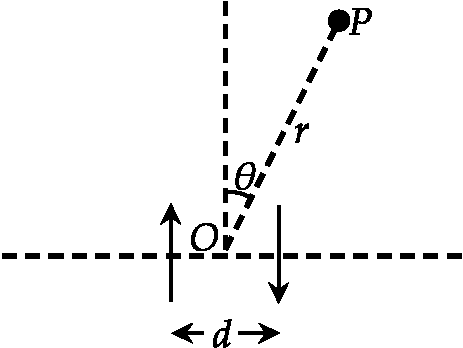
\includegraphics[height=3.2cm,width=5cm]{ED21}
	\end{figure}
	\begin{tasks}(2)
		\task[\textbf{a.}]$d \sin \theta=\left(n+\frac{1}{2}\right) \lambda$
		\task[\textbf{b.}]$d \sin \theta=n \lambda$
		\task[\textbf{c.}] $d \cos \theta=n \lambda$
		\task[\textbf{d.}] $d \cos \theta=\left(n+\frac{1}{2}\right) \lambda$
	\end{tasks}
\begin{answer}$\left. \right. $
	\begin{figure}[H]
		\centering
		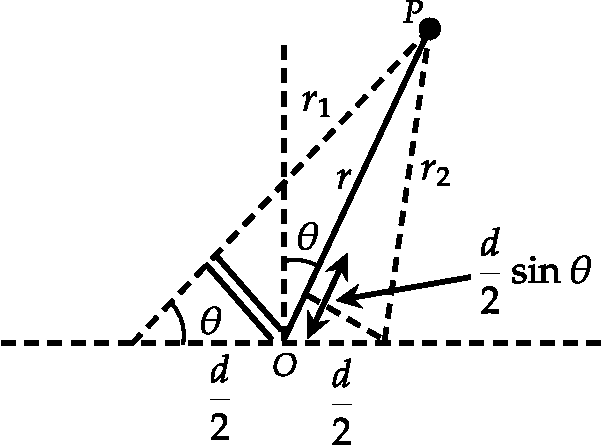
\includegraphics[height=4.5cm,width=6cm]{diagram-20211028(11)-crop}
	\end{figure}
	\begin{align*}
	\intertext{Since dipole are in opposite direction, initial phase
		change will be $\pi$.}
	\text{Thus, }(\Delta \phi+\pi)&=\frac{2 \pi}{\lambda}\text{ (path difference) }=\frac{2 \pi}{\lambda}(d \sin \theta)\\
	\Rightarrow 2 n \pi+\pi&=\frac{2 \pi}{\lambda} d \sin \theta \Rightarrow d \sin \theta=\left(n+\frac{1}{2}\right) \lambda\\
	&(n=0,1,2, \ldots .)\\
	r_{1}&=r+\frac{d}{2} \sin \theta, r_{2}=r-\frac{d}{2} \sin \theta
	\end{align*}
	So the correct answer is \textbf{Option (a)}
\end{answer}
\end{enumerate}
\colorlet{ocre1}{ocre!70!}
\colorlet{ocrel}{ocre!30!}
\setlength\arrayrulewidth{1pt}
\begin{table}[H]
	\centering
	\arrayrulecolor{ocre}
	\begin{tabular}{|p{1.5cm}|p{1.5cm}||p{1.5cm}|p{1.5cm}|}
		\hline
		\multicolumn{4}{|c|}{\textbf{Answer key}}\\\hline\hline
		\rowcolor{ocrel}Q.No.&Answer&Q.No.&Answer\\\hline
		1&\textbf{a} &2&\textbf{d}\\\hline 
		3&\textbf{d} &4&\textbf{c} \\\hline
		5&\textbf{c} &6&\textbf{a} \\\hline
		7&\textbf{a}&8&\textbf{c}\\\hline
		9&\textbf{a}&10&\textbf{b}\\\hline
		11&\textbf{d} &12&\textbf{d}\\\hline
		13&\textbf{a}&14&\textbf{c}\\\hline
		15&\textbf{a}&16&\textbf{d} \\\hline
		17&\textbf{b}&18&\textbf{b}\\\hline
		19&\textbf{d}&20&\textbf{b}\\\hline
		21&\textbf{c} &22&\textbf{a}\\\hline
	\end{tabular}
\end{table}


\newpage
\begin{abox}
	Practise Set-2
\end{abox}
\begin{enumerate}
	\begin{minipage}{\textwidth}
		\item   The electric and the magnetic field $\vec{E}(z, t)$ and $\vec{B}(z, t)$, respectively corresponding to the scalar potential $\phi(z, t)=0$ and vector potential $\vec{A}(z, t)=\hat{i} t z$ are
		\exyear{GATE 2012}
	\end{minipage}
	\begin{tasks}(2)
		\task[\textbf{a.}] $\vec{E}=\hat{i} z$ and $\vec{B}=-\hat{j} t$
		\task[\textbf{b.}]$\vec{E}=\hat{i} z$ and $\vec{B}=\hat{j t}$
		\task[\textbf{c.}]$\vec{E}=-\hat{i} z$ and $\vec{B}=-\hat{j t}$
		\task[\textbf{d.}]$\vec{E}=-\hat{i} z$ and $\vec{B}=-\hat{j} \mathrm{t}$
	\end{tasks}
\begin{answer}
	\begin{align*}
	\vec{E}&=-\vec{\nabla} \phi-\frac{\partial \vec{A}}{\partial t}=-\frac{\partial \vec{A}}{\partial t}=-\hat{i} z,\\\vec{B}&=\vec{\nabla} \times \vec{A}=+\hat{j} t
	\end{align*}
	So the correct answer is \textbf{Option (d)}
\end{answer}
	\begin{minipage}{\textwidth}
		\item If the vector potential $\vec{A}=\alpha x \hat{x}+2 y \hat{y}-3 z \hat{z}$, satisfies the Coulomb gauge, the value of the constant $\alpha$ is
		\exyear{GATE 2015}
	\end{minipage}
\begin{answer}
	\begin{align*}
	\text{	Coulomb gauge condition }\vec{\nabla} \cdot \vec{A}&=0 \Rightarrow \alpha+2-3\\&=0 \Rightarrow \alpha=1
	\end{align*}
\end{answer}
	\begin{minipage}{\textwidth}
		\item Consider magnetic vector potential $\tilde{A}$ and scalar potential $\Phi$ which define the magnetic field $\vec{B}$ and electric field $\vec{E}$. If one adds $\vec{\nabla} \lambda$ to $\vec{A}$ for a well-defined $\lambda$, then what should be added to $\Phi$ so that $\vec{E}$ remains unchanged up to an arbitrary function of time, $f(t)$ ?
		\exyear{JEST 2017}
	\end{minipage}
	\begin{tasks}(4)
		\task[\textbf{a.}] $\frac{\partial \lambda}{\partial t}$
		\task[\textbf{b.}]$-\frac{\partial \lambda}{\partial t}$
		\task[\textbf{c.}]$\frac{1}{2} \frac{\partial \lambda}{\partial t}$
		\task[\textbf{d.}]$-\frac{1}{2} \frac{\partial \lambda}{\partial t}$
	\end{tasks}
\begin{answer}
	\begin{align*}
	\text{	Coulomb gauge condition }\vec{\nabla} \cdot \vec{A}&=0 \Rightarrow \alpha+2-3\\&=0 \Rightarrow \alpha=1
	\end{align*}
\end{answer}
	\item A long straight wire, having radius $a$ and resistance per unit length $r$, carries a current $I$. The magnitude and direction of the Poynting vector on the surface of the wire is
	{\exyear{GATE 2018}}
	\begin{tasks}(1)
		\task[\textbf{A.}] $I^{2} r / 2 \pi a$, perpendicular to axis of the wire and pointing inwards
		\task[\textbf{B.}]$I^{2} r / 2 \pi a$, perpendicular to axis of the wire and pointing outwards
		\task[\textbf{C.}]$I^{2} r / \pi a$, perpendicular to axis of the wire and pointing inwards
		\task[\textbf{D.}]$I^{2} r / \pi a$, perpendicular to axis of the wire and pointing outwards
	\end{tasks}
\begin{answer}
	\begin{align*}
	|\vec{S}|=\frac{1}{\mu_{0}}|(\vec{E} \times \vec{B})|&=\frac{1}{\mu_{0}} \frac{V}{l} \times \frac{\mu_{0} I}{2 \pi a}\\&=\frac{I R}{l} \times \frac{I}{2 \pi a}\\
	\because V&=I R, r=\frac{R}{l} \Rightarrow|\vec{S}|\\&=\frac{I^{2} r}{2 \pi a}
	\end{align*}
	So the correct answer is \textbf{Option (a)}
\end{answer}
	\item  An electromagnetic field is given by
	$$
	\vec{E}(\vec{r}, t)=-\frac{1}{4 \pi \in_{0}} \frac{q}{r^{2}} \theta(v t-r) \dot{r}, \quad \vec{B}(\vec{r}, t)=0
	$$
	where $\theta(x)= \begin{cases}1 & \text { for } x>0 \\ 0 & \text { for } x \leq 0\end{cases}$
	The corresponding charge density $\rho$ and current density $\vec{J}$ are given by
	{\exyear{ JEST-2020}}
	\begin{tasks}(1)
		\task[\textbf{a.}]$\rho=-q \delta^{3}(\vec{r}) \theta(v t-r)+\frac{q}{4 \pi r^{2}} \theta(v t-r) ; \vec{J}=0$
		\task[\textbf{b.}]$\rho=-q \delta^{3}(\vec{r}) \theta(v t-r) ; \vec{J}=0$
		\task[\textbf{c.}]$\rho=\frac{q}{4 \pi r^{2}} \delta(v t-r) ; \vec{J}=\frac{q v}{4 \pi r^{2}} \delta(v t-r) \hat{r}$
		\task[\textbf{d.}] $\rho=-q \delta^{3}(\vec{r}) \theta(v t-r)+\frac{q}{4 \pi r^{2}} \delta(v t-r) ; \vec{J}=\frac{q v}{4 \pi r^{2}} \delta(v t-r) \hat{r}$
	\end{tasks}
\begin{answer}
	\begin{align*}
	\because \vec{\nabla} \cdot \vec{E}&=\frac{\rho}{\varepsilon_{0}} \Rightarrow \rho=\varepsilon_{0}(\vec{\nabla} \cdot \vec{E}) \Rightarrow \rho=-\frac{q}{4 \pi} \vec{\nabla} \cdot\left\{\theta(v t-r) \frac{\hat{r}}{r^{2}}\right\}\\
	\Rightarrow \rho&=-\frac{q}{4 \pi}\left[\theta(v t-r) \vec{\nabla} \cdot\left(\frac{\hat{r}}{r^{2}}\right)+\frac{\hat{r}}{r^{2}} \cdot \vec{\nabla}\{\theta(v t-r)\}\right]\\
	\Rightarrow \rho&=-q \delta^{3}(r) \theta(v t-r)+\frac{q}{4 \pi r^{2}} \delta(v t-r) \quad \because \vec{\nabla} \cdot\left(\frac{\hat{r}}{r^{2}}\right)=4 \pi \delta^{3}(r)\\
	\text { and } \theta(x)&= \begin{cases}1 & \text { for } x>0 \\ 0 & \text { for } x \leq 0\end{cases}\\
	\because \vec{\nabla} \times \vec{B}&=\mu_{0} \vec{J}+\mu_{0} \varepsilon_{0} \frac{\partial \vec{E}}{\partial t} \Rightarrow \vec{J}=-\varepsilon_{0} \frac{\partial \vec{E}}{\partial t} \quad \because \vec{B}=0\\
	\Rightarrow \vec{J}&=-\varepsilon_{0} \frac{\partial \vec{E}}{\partial t}=-\varepsilon_{0} \times \frac{q}{4 \pi \varepsilon_{0} r^{2}} \frac{\partial \theta}{\partial t} \times v \hat{r} \Rightarrow \vec{J}=\frac{q v}{4 \pi r^{2}} \delta(v t-r) \hat{r}
	\end{align*}
		So the correct answer is \textbf{Option (d)}
\end{answer}
	\item  Consider magnetic vector potential $\vec{A}$ and scalar potential $\Phi$ which define the magnetic field $\vec{B}$ and electric field $\vec{E}$. If one adds $-\vec{\nabla} \lambda$ to $\vec{A}$ for a well-defined $\lambda$, then what should be added to $\Phi$ so that $\vec{E}$ remains unchanged up to an arbitrary function of time, $f(t)$ ?
	{\exyear{ JEST-2017}}
	\begin{tasks}(4)
		\task[\textbf{a.}]$\frac{\partial \lambda}{\partial t}$
		\task[\textbf{b.}]$-\frac{\partial \lambda}{\partial t}$
		\task[\textbf{c.}] $\frac{1}{2} \frac{\partial \lambda}{\partial t}$
		\task[\textbf{d.}]  $-\frac{1}{2} \frac{\partial \lambda}{\partial t}$
	\end{tasks}
\begin{answer}
	\begin{align*}
	\intertext{Consider Gauge Transformation}
	\vec{A}^{\prime}=\vec{A}-\vec{\nabla} \lambda=\vec{A}+\vec{\nabla}(-\lambda) \quad \text { and } \quad \Phi^{\prime}=\Phi-\frac{\partial(-\lambda)}{\partial t}=\Phi+\frac{\partial \lambda}{\partial t}
	\end{align*}
		So the correct answer is \textbf{Option (a)}
\end{answer}
	\item  The electric and magnetic field caused by an accelerated charged particle are found to scale as $E \propto r^{-n}$ and $B \propto r^{-m}$ at large distances. What are the value of $n$ and $m$ ?
	{\exyear{ JEST-2013}}
	\begin{tasks}(2)
		\task[\textbf{a.}]$n=1, m=2$
		\task[\textbf{b.}]$n=2, m=1$
		\task[\textbf{c.}]$n=1, m=1$
		\task[\textbf{d.}]$n=2, m=2$
	\end{tasks}
\begin{answer}
	\begin{align*}
	\text { For large distance } F&=\frac{q a \sin \theta}{r}, B=\frac{q a \sin \theta}{r} \Rightarrow E \propto \frac{1}{r}, B \propto \frac{1}{r}\\
	\text { So } m&=n=1
	\end{align*}
		So the correct answer is \textbf{Option (c)}
\end{answer}
	\item  An electron is executing simple harmonic motion along the $y$-axis in right handed coordinate system. Which of the following statements is true for emitted radiation?
	{\exyear{ JEST-2014}}
	\begin{tasks}(1)
		\task[\textbf{a.}]The radiation will be most intense in $x z$ plane
		\task[\textbf{b.}] The radiation will be most intense in $x y$ plane
		\task[\textbf{c.}]The radiation will violate causality
		\task[\textbf{d.}] The electron's rest mass energy will reduce due to radiation loss
	\end{tasks}
\begin{answer}
Oscillating electron does not emit radiation in the direction of oscillation.
In the perpendicular direction of oscillation intensity is maximum.
So in this case the intensity will be maximum along $x$ and $z$ - axis or $x z$-plane (intensity is also en $x y$-plane but less).\\
	So the correct answer is \textbf{Option (a)}
\end{answer}
\end{enumerate}